  \documentclass[a4paper, 12pt]{report}

\usepackage{amsfonts} % if you want blackboard bold symbols e.g. for real
\usepackage{graphicx} % if you want to include jpeg or pdf pictures
\usepackage{lmodern}
\usepackage{amsmath}
\usepackage{amssymb}
\usepackage{algorithmic}
\usepackage{algorithm}
 %%% Time-stamp: <mainrep.tex 13:08, 25 May 2009 by P. Sunthar>

%%% $Log:$




%%% Some commonly used packages (make sure your LaTeX installation
%%% contains these packages, if not ask your senior to help installing
%%% the packages)

\usepackage[bookmarks,%
            a4paper,%
            breaklinks,%
            backref=false,%
            dvips,ps2pdf,%
            pdfhighlight=/I,%
            pdffitwindow=true,%
            pdfstartview=Fit,%
            pdfcenterwindow=true,%
            linkbordercolor={1 0 1},%
            %colorlinks,%
            pdftitle=Progress report%
            pdfauthor=Kim Svensson]%
            {hyperref}



\usepackage{amsmath}
\usepackage{epstopdf}
\usepackage{natbib}
\usepackage{booktabs}
\usepackage{graphicx}
\graphicspath{{expt/}}
\usepackage{setspace}
\usepackage{natbib}
\usepackage{times}
\usepackage[varg]{txfonts}
\usepackage[utf8]{inputenc}

%%% Macro definitions for Commonly used symbols
\newcommand{\etas}{\ensuremath{\eta_{\mathrm{s}}}}
\newcommand{\tdegree}{A project progress report submitted for the award of\\}
\newcommand{\degree}{\tdegree MEng Computer Science\\*}
\newcommand{\texam}{Second examiner: }
\newcommand{\exam}{\texam Dr Srinandan Dasmahapatra}
\newcommand{\tsupervisor}{Project supervisor: }
\newcommand{\supervisor}{\tsupervisor Dr.\ Sarvapali D. Ramchurn}
\newcommand{\school}{Electronics and Computer Science \\*
Faculty of Physical and Applied Sciences\\*
University of Southampton\\*}


\newenvironment{changemargin}[2]{%
\begin{list}{}{%
\setlength{\topsep}{0pt}%
\setlength{\leftmargin}{#1}%
\setlength{\rightmargin}{#2}%
\setlength{\listparindent}{\parindent}%
\setlength{\itemindent}{\parindent}%
\setlength{\parsep}{\parskip}%
}%
\item[]}{\end{list}}


\begin{document}

\author{Kim Svensson}
\date{\today}
\title{Combinatorial optimization of NP-hard problems using dynamic GPU
programming}

\makeatletter
\begin{titlepage}
\begin{changemargin}{-2cm}{-2cm}
\begin{center}
\LARGE\school %

\LARGE
\vfill
\@author \\*
\@date \\*
\doublespacing
\@title \\*
\vfill
\singlespacing
\supervisor \\*
\exam \\*
\vfill
\degree
\end{center} 
\end{changemargin}
\end{titlepage}
\makeatother

\pagenumbering{arabic}
\begin{abstract}
We develop the first parallel algorithm for Coalition Structure Generation
(CSG), which is central to many multi-agent systems applications. Our approach
involves distributing the key steps of a dynamic programming approach to CSG
across computational nodes on a Graphics Processing Unit (GPU) such that each of
the thousands of threads of computation can be used to perform small
computations that speed up the overall process. In so doing, we solve important
challenges that arise in solving combinatorial optimisation problems on GPUs
such as the efficient allocation of memory and computational threads to every
step of the algorithm. In our empirical evaluations on a standard GPU,  our
results show an improvement of orders of magnitude over current dynamic
programming approaches with an ever increasing divergence between the CPU and
GPU-based algorithms in terms of growth. Thus, our algorithm is able to solve
the CSG problem for 29 agents in just under 10 minutes as opposed to three
days for the current state of the art dynamic programming algorithms.

\end{abstract}
\tableofcontents
\newpage

\section{Introduction}
\noindent Coalition formation is one of the key coordination mechanisms in
multi-agent systems. It involves the coming together of a number of  agents to
achieve some individual or group objective.  An important step in the 
 coalition formation process involves partitioning the set of agents into
coalitions that, on aggregate (as a coalition structure), maximise the
efficiency in the system. This problem is termed the 
\emph{Coalition Structure Generation} problem (CSG)
~\cite{DBLP:journals/ai/SandholmLAST99}.   The  CSG problem is a hard
combinatorial optimisation problem and scales in $\omega(n^n)$
\cite{DBLP:journals/ai/SandholmLAST99}. To date, many algorithms have been
designed to solve the CSG. These range from branch-and-bound approaches such as
\cite{rahwan2009anytime}, to dynamic programming approaches such as
\cite{DBLP:conf/atal/RahwanJ08,rahwan:jennings:2008b}. The latter are
particularly attractive given their lower complexity, but most of these
algorithms scale to around 30 agents given the exponential growth in computation
involved. We also note that these algorithms were mainly designed for
single-threaded architectures, and even if distributed variants exist
\cite{michalak2010distributed}, these require storing the input data redundantly
across multiple computers and sharing information over network links that may be
liable to delays and losses. 

In contrast, in the last few years, a surge in the development of frameworks for
parallel programming on a single machine has been noted with the development of
general-purpose Graphics Processing Units (GPUs). Indeed, these processors,
originally developed for only processing high end graphics, can now be
programmed to perform simple mathematical operations that, when performed in
thousands in parallel, can significantly outperform single-threaded machines
with higher frequencies. There are multiple challenges,
however, that need to be overcome before complex algorithms as for CSG can be
implemented onto the GPU (elaborated in Section \ref{sec:gpu-csg})
including the need to limit random memory access,  the limits on the number of
threads that can be launched to share the same memory blocks, and the need to
avoid loading data frequently from main memory. 

Against this background, in this paper, we present a parallel algorithm for CSG
for highly multi-threaded GPUs that meets the challenges above and outperforms
the best algorithms for CSG. The algorithm, GPU-CSG, parallelises the
computation of individual steps of a dynamic program to solve the CSG. It does
so by partitioning the computation across thousands of threads where each solves
a small sub-problem of the larger optimisation problem. The solution to each
sub-problem is then used to find the best partition of agents. In more detail,
this paper advances the state of the art in the following ways. First, we
develop the first parallel  algorithm for CSG that avoids redundant memory
storage and inter-processor communication. Second, we prove that GPU-CSG is
correct and complete and demonstrate through empirical evaluation that its
growth rate is significantly lower than that of the dynamic programming approach
it builds upon. Third, we empirically show that GPU-CSG outperforms the state of
the art by 
orders of magnitude, solving the CSG problem for 29 agents in less than 10
minutes
as opposed to 83 hours for the CPU-based algorithm.

The rest of this paper is structured as follows. Section 2 presents the
background to this work and discusses related work, as well introduces the
the GPU architecture and details the DP algorithm. Section 3 and 4 then details
the GPU-CSG which is built upon the DP algorithm,
while Section 5 concludes.


\section{Background}
\subsection{Combinatorial Auctions}
Sometimes auctioneers may sell out several of their assets at the same time such
as the government selling parts of the radio spectrum. The bidder may then make
offers on subsets of the assets. The problem occurs when there is a large amount
of assets being sold while the amount of bids are non-trivial. As for each bid, 
it have to made sure that no other bid that only acquires a subset of the
original bid is greater.
The goal is therefore to calculate which set of pairwise disjoint bids gives the
most revenue to the auctioneer.\\*
 Consider that the auctioneer is selling the assets $f_0 , f_1$
and $f_2$. The bids collected are as following:

\begin{table}[htb]
\centering
\begin{tabular}{ l | c}
\hline  
Set & Bid \\
\hline
$f_0$ & 3 \\
$f_1$ & 2 \\
$f_2$ & 6 \\
$f_0, f_1$ & 7 \\
$f_0, f_2$ & 7 \\
$f_1, f_2$ & 4 \\
$f_0, f_1, f_2$ & 6 \\
\end{tabular}
\caption{This table shows some data}
\label{tab:bids}
\end{table}
The winning bid configuration would be the following set:$
\{\{f_2\},\{f_0 , f_1\}\}$ 
with a total sum of $7 \{f_0 , f_1\}+6 \{f_2\} = 13$ as it
is the maximum sum of all combinations of disjoint sets. Where all complete
disjoints sets are:

\begin{table}[htb]
\centering
\begin{tabular}{c | l }
\hline
Complete disjoint set & Sum\\
\hline
$\{\{f_2 \},\{f_0 , f_1 \}\} $ & 13 \\
$\{\{f_1 \},\{f_0 , f_2 \}\} $ & 9 \\
$\{\{f_0 \},\{f_1 , f_2 \}\} $ & 7 \\

$\{\{f_0,f_1 , f_2 \}\} $ & 6 \\
$\{\{f_0 \},\{f_1 \}, \{ f_2 \}\} $ &  11
\end{tabular}
\caption{This table shows some data}
\label{tab:disjoint}
\end{table}

The way you calculate the optimal solution for combinatorial auctions is by
given any set, 
find the greatest sum for the whole collection of pairwise disjoint subsets of
that set and evaluate if it is greater than the set itself.
This procedure is done for all sets to finally find a final solution that is the
optimal one which give the largest revenue to the auctioneer.
\subsection{Coalition Structure Generation}
Coalition structure generation is a complete analogy to combinatorial auction
but from another perspective.
It can be translated in such that the assets become agents, 
an agent can be described as a entity that act on its own, be it a person or a
node in a network.
A set of assets subjected to a bid is called a coalition formation, 
in short when two or more agents form a coalition to be regarded as one entity.
The auction bid will be translated to coalition value, 
which means the value gained when two or more agents form a coalition.
Analogous to the previous example, given N agents, 
generate a set of coalition formations such that the outcome is optimal in
regards to the coalition formation value.
This however will be an extreme challenge as the number of possible partitions
grows exponential with $n$, specifically $O(n^n)$~\cite{eps265062}.
One algorithm to solve this problem in $O(n^3)$ time is called the Dynamic
Programming(DP) algorithm~\cite{DPalgorithm} described in
algorithm ~\ref{DP}.

It works with the dynamic programming bottom-up approach where you start at sets
with cardinality 2 and see if the sum of the pair-wise disjoint subsets value is
greater than the original set.
If it is assign the new sum to that set.
With this principle, 
all sets with the greatest sum will be carried forward when the cardinality of
the sets increases.
This algorithm is deterministic, 
meaning that even if there is only one bid, the computation will take the same
time as 1000 bids for a given set of agents. \\

\subsection{Previous Work}
Solving data-independent and parallel problems will always have a benefit when
run on a GPU, 
whether it is computing on MRI scans, which gave a significantly large speedup
factor of 431 using the GPU, 
or generating hashes and getting a comparably modest speedup of times
11~\cite{ryoo2008optimization}.  
This is particularly the case whenever the algorithm has data-independent
sub-routines which may be run concurrently. 
If so the GPU will most likely perform better. 
Combining the GPU together with dynamic programming has been used before to
solve similar combinatorial optimisation problems.  
Boyer, et al. successfully implemented and solved the knapsack problem with a
factor speedup of 26~\cite{boyer2012solving}.  
They also introduced ways to reduce memory usage and thus enable computation of
much larger data sets, as well as reduce the  bandwidth utilised. 
In so doing, they also reduce computation time by being able to fetch more data
points at an faster rate. 
Thus, they fully exploit the key features of GPU programming whereby, with
limited amount of memory available on a GPU,  
they are able to maximise the effective bandwidth of the algorithm.

Now, turning to the CSG problem, in terms of parallel programming approaches, 
we note the work of Michalak et. al. that uses a distributed variant of the
anytime IP algorithm called 
D-IP to solve the Coalition Structure
Generation~\cite{michalak2010distributed}. 
They use 14 dual-core workstations to distribute the workload to speed up their
run-time. 
Their algorithm  shows it is possible to distribute the solutions for the CSG
problem and that there may be
significant from distributing computation (taking only 11\% to 4\% of the time,
compared to the centrilised and serialised IP). 
However, while their algorithm use traditional programming strategies effective
on powerful single-threaded systems, 
it does require data to be shared between computational nodes over potentially
slow Ethernet links and also sharing 
redundant copies of the input across each. Finally, their algorithm also suffers
from the same weaknesses as IP, that is, 
no deterministic completion time (in the worst case ($O(n^n))$ as it is
dependent on the coalition value function. 
In contrast, GPU-CSG has a deterministic completion time ($O(3^n)$) and relies
on much faster GPU memory access.

As shown, GPUs have assisted largely while solving problems ranging from
relatively data-independant algorithms to more complex problems in the field of
combinatorial optimisation. While researchers have only tackled the
combinatorial auction problems only with the use of a handful of machines
trying to spread
the workload. No one have to this date tackled the coalition structure
generation problem using GPUs.

In what follows, we first describe the CUDA architecture (the GPU architecture
provided by NVIDIA) to clarify what 
are the key features and issues of using GPUs to solve large combinatorial
problems.
We then describe the DP algorithm and the data structures we use to implement it
on the CUDA architecture.

\subsection{The CUDA Architecture} \label{Cuda} %done
Graphics Processing Units (GPUs) from NVIDIA and AMD are highly multi-threaded,
many-core architectures primarily 
aimed at highly parallel image processing and rendering. In recent years,
however, 
there has been a move to use these to support more general-purpose computing
through the OpenCL and NVIDIA CUDA framework.
This was achieved by devoting a larger amount of transistors towards many
computational units rather than data caching and advanced 
flow control more often seen in CPU architectures. NVIDIA describes their
general-purpose GPU CUDA architecture as a Single Instruction 
Multiple Threads (SIMT) architecture, meaning groups of multiple threads execute
the same instructions concurrently and is proportional to SIMD architectures. 
This enables their GPUs to be highly advantageous when performing
data-independent and non-divergent tasks. 
To understand this further the grouping of the threads need to be explained and
is outlined in figure \ref{fig:reduction}.
\begin{figure*}
\centering
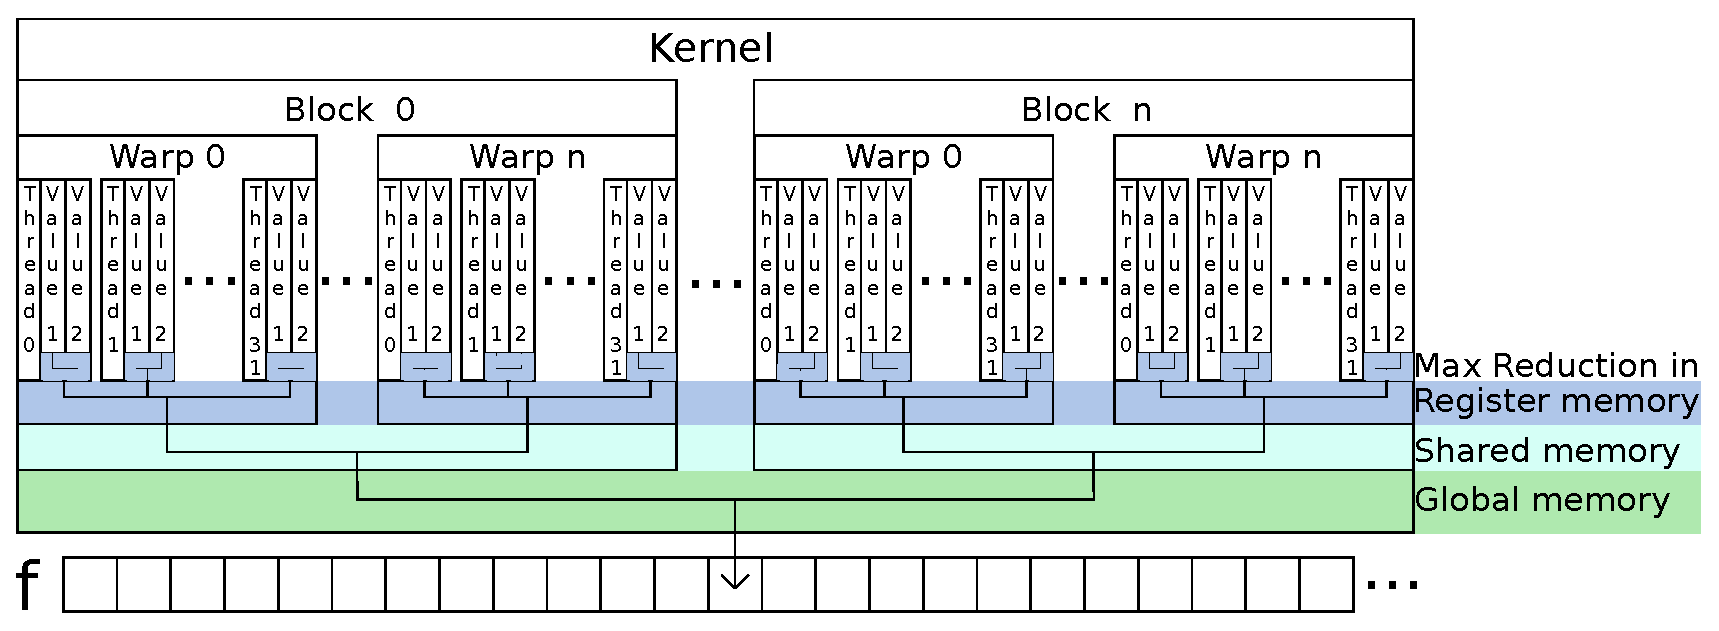
\includegraphics[width=\linewidth]{reduction}
\caption{Outline of the memory hierarchy and scope
\label{fig:reduction}. The kernel is a function called by the Host}
\end{figure*}
The kernel is a device-specific CUDA function that is called by the sequential
host code(CPU), 
which will request a specified number of blocks in a grid of blocks. 
Each block may to this date consist of up to 1024 threads depending on the
compatibility of the card, 
with a maximum block grid size of $2^{31}-1$ blocks subjected to compatibility. 
When run, the blocks will be distributed onto available multiprocessors, which
then independently schedule the run-time of the block. 
Note that blocks may be executed concurrently or sequential depending on the
current workload and the number of available multiprocessors. 
The block is split into smaller units of 32 threads called warps, all threads
within the same warp are always scheduled the same instruction 
to be run and this is what embodies the SIMT \footnote{Single Instruction
Multiple Threads (SIMT) architecture, All threads inside a warp execute the same
instruction} paradigm. 
Therefore, branching threads causing intra-warp divergence means a warp will
have inactive threads not executing any instructions,  which may lead to poor
efficiency with worst case of sequential performance. 
Further, warps are scheduled independently of each other meaning possibility of
concurrent warp execution.

The threads communicate with each other through writes to various types of
memory outlined in table \ref{mem} and figure \ref{fig:reduction}. 
There are three types of thread writable memory in the architecture; registers
and local memory are each threads coupled memory, 
which is not volatile and may be shared with other threads inside the same warp
as described in Section \ref{reduction}. 
Shared memory is as its name tells is shared between all threads within the same
block, as it may be written to by any thread 
within the block it should be treated as volatile, thus synchronization inside
the block have to be consider whilst dealing with shared memory.
Finally, global memory is the only persistent memory, which will persist between
each kernel call, it may be manipulated by the host, 
but also by any thread, and is the only means of communication in between
kernels, blocks, and the host.

Now, an important element of GPU programming is to manage the access to global
memory effectively as it is very slow compared to memory access 
of the on-chip memory on the GPU. In more detail, each load request from memory
will fetch in cache-lines of size $32*wordsize$, meaning 
cache-lines of 32, 64, and 128 bytes each when pulling the primitives char,
short and int respectively. 
This is because, as mentioned earlier, all 32 threads within the same warp issue
the same instruction. 
Thus each warp fetches 32 entities of a specific word type, if the memory reads
within a warp is not coalesced (grouped within the same cache-line)
within consecutive words, the effective bandwidth will drop immediately. 
Table \ref{mem} summarises the key features of GPU memory access speeds and
shows why it is important to avoid loading data from the global memory.

\begin{table}
\centering
\caption{Memory scope, lifetime, and speed \label{mem}}
\begin{tabular}{|l|l|l|l|} \hline
Type&Scope&Lifetime&Relative Speed \\ \hline
Register&Thread \& Warp&Thread&Fastest\\
Shared&Block&Block&Fast\\
Global&Kernel \& Host&Program&Slow\\
\hline\end{tabular}
\end{table}
In the next subsection, we describe the DP algorithm, which we build upon.

\subsection{The {DP} Algorithm} 
%done
The DP algorithm \cite{DPalgorithm} was originally designed to solve the winner
determination problem for combinatorial auctions. However, in recent years, it
has been applied as the de facto  algorithm (complete and with the lowest worst
case complexity) to solve the CSG problem and variants of it have improved and
adapted it to different settings
\cite{DBLP:conf/atal/RahwanJ08,DBLP:conf/aamas/VoiceRJ12}. However, the core of
the algorithm is the same in all these variants and relies on dynamic
programming. Hence, in this paper we use this as the basis for our GPU version
as the dynamic programming approach has shown potential for parallelisation as
evidenced by previous work (as for the Knapsack problem as mentioned earlier). 

To show how the algorithm works, we first formalise the CSG problem.  Let
$A=\{1,\ldots,\vert A \vert \}$ be a set of agents. A subset $C \subseteq A$ is
termed a coalition.  Then, a $CSG$ problem is completely defined by its
characteristic function $v: 2^{A} \rightarrow \Re$ (with $v(\emptyset)=0$),
which assigns a real value representing utility to every feasible coalition. 
The CSG problem is to identify the exhaustive disjoint partition of the space of
agents into coalitions (or, \emph{coalition structure})  $CS=\{C_1,\ldots,C_k\}$
so that the total sum of values, $\sum^k_{i=1} v(C_k)$,
is maximised.

Now, DP (see Algorithm  \ref{DP}) works by producing two output tables, $O$ and
$f$, 
where each table has one entry per coalition structure. 
An entry in $f$ represents a value a certain coalition structure is given, 
while $O$ represent which splitting, if any, maximised the coalition structure
for the entry in $f$ that it represents.
More elaborated, given all coalitions of agents $C\subseteq A$, for each
coalition in $C$, evaluate all
pairwise disjoint subsets (here named splittings) on their pairwise collective
sum against the coalitions
original value. Given one splitting is greater, update the value of the
coalition $f(C) := f(C') + f(C\setminus C')$
and assign $O$ on $C$ to represent the new splitting, $O(C) := \{C',C\setminus
C'\}$. These steps are first carried out on all coalition structures with two
agents, continuing until $|A|$ agents.  This means, given a coalition structure
$S$ with cardinality $|S| = n$, then all coalition structures
for the sizes $1,2,...,n-1$ have already been evaluated. The dynamic programming
algorithm is entirely deterministic meaning that even if there was only one or
two valuations, the algorithm will evaluate all splittings before it reaches a
conclusion. However this algorithm does not work well with a large number of
agents as it grows exponentially and has time and memory complexity $O(3^n)$. As
described later in Section \ref{algorithm}, the part of the algorithm that is
parallelized is the max function on line \ref{lst:line:a}, which handles the
evaluation of all splittings of a given coalition structure.

The table $O$ may be discarded and not calculated to reduce memory requirements
by half removing instant access to the final splittings. These final splittings
are easily retrieved as outlined in algorithm \ref{idpref}.  Essentially, all
coalitions in $C \in CS^*$ whose value in $f$ is not equal to the initial value
in $v$, find the first splitting that is equal to the value in $f$. The overhead
of this is insignificant as it needs to evaluate at most $n -1$ coalitions
compared to the exponential
number of evaluations carried out in the previous steps\cite{eps265062}.

\begin{algorithm}
\caption{Dynamic Programming algorithm \label{DP}}
INPUT: $b(C)$ the bids for all sets $C \subseteq A$ where $A$ is the set of
assets.\\*
VARIABLES: $f$ a function that maps from a subset $C \subseteq A$ to a value\\*
$O$ a function that maps from a subset $C \subseteq A$ to the subset that
maximize the value for set $C$.
\begin{algorithmic}[1]
\STATE\algorithmicfor\ all $x \in A$, \algorithmicdo $f(\{x\}):=
b(\{x\}),O\{x\}:= \{x\}$ \algorithmicendfor
\FOR{$i := 2$ to $n$}
\FOR{all $C \subseteq A: \vert C \vert == i$}
\STATE $f(C) := max\{f(C\backslash C')+f(C'):C'\subseteq C \wedge 1 \leq \vert
C' \vert \leq \dfrac{\vert C \vert}{2}\}$ \label{lst:line:a}
\STATE\algorithmicif $f(C) \geq b(C)$ \algorithmicthen\ $O(C) := C^{*}$ \hfill
Where $C^{*}$ maximizes right hand side of line~\ref{lst:line:a}
\algorithmicendif
\STATE\algorithmicif $f(C) < b(C)$ \algorithmicthen\ $f(C) := b(C)\wedge O(C) :=
C$ \algorithmicendif
\ENDFOR
\ENDFOR
\end{algorithmic}
\end{algorithm}


\begin{algorithm}
\caption{Enumeration of the optimal splittings through re-evaluation of small
amount of coalitions \label{idpref}}
INPUT: $v:$ array of the initial bids for all coalitions $C \subseteq A$. 
$f:$ the final evaluated values gathered from evaluating splittings.
\begin{algorithmic}[1]
\STATE Set $CS^* := \{A\}$
\FOR{all $C \in CS^*$} \label{lst:line:redo2}
\IF{$f(C) \neq v(C)$}
\STATE find first $C^*$ where $f(C) = f(C\backslash C^*)+f(C^*):C^*\subseteq C
\wedge 1 \leq \vert C^* \vert \leq \dfrac{\vert C \vert}{2}$ \label{lst:line:aa}
\STATE Set $CS^* := (CS^*\setminus \{C\})\cup \{C^*,C\setminus C^*\}$
\STATE Goto \ref{lst:line:redo2} and start with a new $CS^*$
\ENDIF
\ENDFOR
\RETURN $CS^*$
\end{algorithmic}
\end{algorithm}
Having described the DP algorithm, we next elaborate on the data structure we
use to extend DP into GPU-CSG and then go on to detail the algorithm.


\section{Work}

%\begin{algorithm}
%\caption{Calculate the }asd

\subsubsection{GPU-CSG} \label{sec:gpu-csg} %done
GPU-CSG parallelises the key steps of the DP algorithm. This is a non-trivial
process (as we will see) as it requires us to be efficient in memory access and
in sharing the computation among the threads on the GPU so that access to global
memory is reduced while minimising the need for synchronising the threads. To
this end, we first propose a memory efficient technique to store coalitions and
their values in memory. This is important because (as discussed  in Section 2),
the GPU typically have relatively smaller amounts of memory. Moreover, we
discuss different ways to navigate through the search space of coalitions as DP
requires splitting coalitions into their components to evaluate each sub-problem
separately.
\subsubsection{The Data Structure}\label{sec:data}
How data is represented and structured is important, especially in bandwidth
bound algorithms where the majority of time is spent fetching data from memory
and the arithmetic overhead is low.
Selecting the right composition will reduce the memory requirements
substantially. Given the two entities of data that are needed to be represented
for each coalition structure, the coalition structure itself and its value in
$f$, we propose data structures that aim to allow a large number of agents to be
represented in spite of the exponential growth of the input (i.e., $2^n$).

In order to minimize memory usage we applied several techniques as follows.
First, we represent each coalition as a fixed sized array of values, where each
value represents a distinct agent. While this may seem intuitive at first, if
the members are represented as bits set in a fixed sized integer, the memory
requirement will be reduced substantially as shown by previous
studies~\cite{boyer2012solving}.
When solving the CSG problem with $n$ agents representing members as an array of
values, there are \[\dbinom{n}{i}\] coalition structures of size $i$, where $i$
entries have to be stored per coalition structure.

The total number of values needed to store just to represent the coalition
structures is therefore equal to:
\begin{displaymath}\sum_{i=i}^{n} \dbinom{n}{i}\times i\end{displaymath}

Given the same constraints, representing the coalition structure as an fixed
sized integer, it is only 
needed to store one entry per coalition, which is all together
\begin{math}2^n-1\end{math} data points.

To give an example, with four agents $A = {f_0,f_1,f_2,f_3}$, the coalition $C =
{f_0,f_2,f_3}$ would be represented as $C = 1101$ in the binary system and $13$
in the decimal system. Therefore, if the coalition structure is represented as
an integer it can implicitly be stored as an index to its coalition value, by
enumerating it at run-time. That means the only memory constraint on the system
is the storage for all coalition values.

Given that the index to the value of a coalition structure is as a binary
representation, the distribution of, coalition structures 
that are lexicographically adjacent with the same cardinality will be evenly
distributed over the fixed sized array.
This rise two constraints. First, the whole fixed sized array have to fit into
the memory of the GPU, limiting the number of agents that can be represented.
Second, fetching values will be in non-coalesced manner causing waste of
bandwidth, which to some degree is resolved by detecting values that can be
shared between coalition structures, as described in Section \ref{sectionsplit}.


Now, having defined coalitions as binary arrays, we next move on to explain how
we create splittings of such coalitions efficiently for our algorithm to go
through sub-solutions of the CSG problem.
\subsubsection{Coalition Structure Splittings}

% \begin{table}
% \centering
% \caption{Initialize shift on $C = \{f_0,f_2,f_3\}$\label{split}}
% \begin{tabular}{|l|r|r|} \hline
% Binary&$1_3 1_2 0_1 1_0$&\\ \hline
% Shift&\vline 0\vline 3\vline 2\vline 0\vline& Result \\ \hline
% Splitting 1 & $0001 : 1 << shift[0]$& $0001$ \\ 
% Splitting 2 & $0010 : 1 << shift[1]$&$ 0100$ \\
% Splitting 3 & $0011 : 1 << shift[0]$&\\ & $+ 1 << shift[1]$&$0101$ \\
% \hline\end{tabular}
% \end{table}

Splittings as mentioned are pairwise disjoint subsets of a coalition structure, 
given the coalition structure $C = \{f_3,f_2,f_0\}$ the splittings
are shown in table \ref{split}. In order to generate the splitting there are
essentially three methods used:  $initShift$, $initialSplit$, and $nextSplit$. 

\begin{table}[htbp]
\centering
\caption{Splittings of $C = \{f_3,f_2,f_0\}$ Binary $C = 1101$ \label{split}}
\begin{tabular}{|l|c|c|c|} \hline
Set& $\{f_0\}$,$\{f_3,f_2\}$ &$\{f_2\},\{f_3,f_0\}$&$\{f_3\},\{f_2,f_0\}$ \\ 
system&&& \\ \hline	
Binary&0001\hfill 1100&0100\hfill 1001&1000\hfill 0101 \\
system&&& \\
\hline\end{tabular}
\end{table}

The function $initShift$, as detailed in Algorithm \ref{initshift} and partly
illustrated in Figure \ref{fig:howitworks}, 
 is necessary to setup the environment for all calls to $initialSplit$.
 It takes as input the coalition structure that should be evaluated and the
index $n$ which
represent the index for the coalition structure in the two dimensional array
$shift$.
\begin{algorithm}
\caption{$initShift$ input $Coalition:C$ $Index:n$ \label{initshift}}
\begin{algorithmic}[1]
\STATE $t :=C$
\STATE $count := 0$
\WHILE{$t > 0$} { 
\STATE $index := FindFirstSet(t)$ \hfill Finds first bit set in t
\STATE $shift_{n,count} := index$ 
\STATE $nullBit(t,index)$ \hfill Sets one bit in t to zero
\STATE $count++$
}
\ENDWHILE
\RETURN shift
\end{algorithmic}
\end{algorithm}
The general idea is to put into the shared $shift$ array which members the
coalition structure have in an ordered fashion. As illustrated in Figure
\ref{fig:howitworks}, the coalition $C = \{f_3,f_2,f_0\}$ will have the values
0, 2 and 3 put in the array, these numbers represent which unique members it
contains. It does so by using the bit operation $Find First Set$ which return
the index of the first set bit, where the index represent which unique member in
the coalition structure. It uses $Find First Set$ to find the first set bit in
the coalition structure, and sets the bits index in the $shift$ array. Remove
that member from the coalition structure by setting that bit to zero and scan
for next set bit again, do so until all members have been identified and the
coalition structure is empty. The two-dimensionality of the $shift$ array is to
have one row in the array for each coalition structure that is being evaluated
by the kernel. 
\begin{figure*}[htbp]
\centering
\includegraphics[width=0.7\linewidth]{test}
\caption{How initShift and initialSplit works\label{fig:howitworks}}
\end{figure*}

Further, using these values with the function $initialSplit$ described in
Algorithm \ref{alg:initalsplit} to generate an initial splitting works as
follows: Given the index $n$ as input that is an ascending integer value, which
represent the $nth$ subset we want to create, and $C^*$ which represent the row
in $shift$ for coalition structure $C$. The idea is to map the  bits set in $n$
to bits in the coalition structure $C$, effectively transforming members of $n$
to members in $C$. It does so by using $Find First Set$ to find the indexes of
set bits in $n$, where the index will eventually represent the $n$th ordered
member of coalition structure $C$. First, take the indexes of bits set in $n$
and use them to reference a column in row $C^*$ in the shift array, this will
yield one member value $v$ from coalition structure $C$. To add that member to
the subset to be created, take a single bit and binary left shift it $v$ places,
and add it to the subset. Remove the set bit in $n$ and continue with previous 
operations until $n$ is empty. 

To illustrate as shown in Figure \ref{fig:howitworks}, the third subset
represented as the binary value of $0011$, have its bits set in the indexes zero
and one. In the shift array for coalition structure $C$, the indexes zero and
one represent the first and secondly ordered members, which is agents $f_0$ and
$f_2$ with values $v$ of 0 and 2. To form the subset, as described earlier, add
together a single bit left shifted 0 places with a single bit left shifted 2
places. This will finally yield the subset $0101$ which have the members $f_0$
and $f_2$ in it. Then to generate the next splitting, a call to $nextSplit$ in
Algorithm \ref{alg:nextsplit} is needed that works through a recurrence relation
to generate the next splitting.

\begin{algorithm}
\caption{ nextSplit input $Coalition:C$ $Splitting:S$\label{alg:nextsplit}}
\begin{algorithmic}[1]
\STATE $C' := twosComplement(C)$
\STATE $S' := bitwiseAND((C'+S),C)$
\RETURN $S'$
\end{algorithmic}
\end{algorithm}

\begin{algorithm}
\caption{initialSplit input $index:n$ $index:C^*$\label{alg:initalsplit}}
\begin{algorithmic}[1]
\STATE $t := n$
\STATE $S := 0$
\WHILE{$t > 0$} { 
\STATE $index := FindFirstSet(t)$ \hfill Finds the first set bit in t
\STATE $S := S + leftShift(1,shift_{C^*,index})$ \hfill Shifts 1 left with the
value in shift and adds
\STATE $nullBit(t,index)$ \hfill Sets the bit of t to 0
}
\ENDWHILE
\RETURN $S$
\end{algorithmic}
\end{algorithm}

\subsubsection{Collisions between Splittings of Coalitions} \label{sectionsplit}
Given that each thread evaluates several splittings over numerous coalition
structures in parallel, 
it is bound that splittings on two coalitions that overlap will have splittings
that collide.
A collision means that splittings of coalition contain at least one identical
subset shared between them.
\begin{displaymath}\forall S\subset C \wedge S' \subset C' : C \cap C' \neq
\emptyset \Rightarrow \exists S \wedge S' : S = S'\end{displaymath}
For all splittings of $C$ and $C'$ where the coalitions intersect, there exist
at least one subset of a splitting shared between them.

The number of splittings that collide is dependent on how many common members
the coalitions have in common.
\begin{displaymath}2^{n}-1:C\neq C'\wedge |C \cap C'| = n \wedge n > 1
\end{displaymath}
Specifically, the number of splittings in common is how many splittings
can be done on all the members of the intersection. Normally, each splitting
would be fetched from global memory resulting in it being fetched several times,
if it have not been evicted from the cache-memory.

For example, given two coalition structures $C_1 =\{f_0,f_1,f_2\}$ and $C_2
=\{f_0,f_1,f_3\}$ that intersect on $f_0$ and $f_1$, all splittings value where
one subset only contain one or both members may be shared in-between them. I.e.
the values for $S_1 = \{f_0\}$, $S_2 = \{f_1\}$, and $S_3 = \{f_0,f_1\}$ are
interchangeable.


By using collision detection as described in here, the
number of redundant fetches may be reduced,
which may only be possible by evaluating two or more coalitions at the same
time. 

\subsubsection{Reduction} \label{reduction} %done
As the evaluation of each coalition  means finding the splitting  of the
coalition  which maximizes the value of the coalition structure, it is simply
needed to compare the values of all splittings with each other to find the
most-valued one.  The reduction is done only on the warp level.
This is done by utilizing a function
called $\_\_shfl\_xor$ which allows for an exchange of register values between
any thread within the same warp.
Using this function, the maximum value within the warp is found.


\subsection{Algorithm}
\subsubsection{The GPU-CSG Algorithm}\label{algorithm}
%\begin{algorithm}[]

\textbf{Input}

$f$\hfill The array which holds the values

$C_0$\hfill The first coalition structure to do evaluation on

$\Psi$\hfill The maximum number of splittings

\textbf{Constants}

$\lambda = \lceil\Psi/32\rceil$ \hfill How many splittings should be evaluated
per thread

$\alpha = 2*\space \# \space warps$ \hfill Total number of coalition structures
evaluated of the block

$tid = threadIdx.x$ \hfill The thread index inside the block

$laneId = tid \% 32$ \hfill The thread index inside the warp

$warpId = tid / 32$ \hfill The warp index inside the block

\textbf{Variables} 

$shift$ \hfill A shared array containing the left shift values for each
coalition

$S$ \hfill The current splitting

$Max$ \hfill The maximum value

$\Delta$ \hfill A shared array containing the coalition structures that will be
evaluated 


$\psi := \lambda*laneId$ \hfill Initial subset construction index



\textbf{Start of algorithm}
\begin{algorithmic}[1]
\IF{$tid = 0$}
  \STATE $\Delta_0 := C_0$ \hfill Thread 0 sets the first coalition from input
  \FOR {$i := 1$ to $\alpha$}
    \STATE $\Delta_{i,0} := nextCoalition(\Delta_{i-1,1})$ \hfill Generate the
next coalitions to evaluate
    \STATE $\Delta_{i,1} := nextCoalition(\Delta_{i-1,0})$ \hfill Generate the
next coalitions to evaluate
  \ENDFOR 
\ENDIF
\STATE $syncthreads()$ \hfill Synchronise the threads inside the block 
\IF{$laneId < 2$}
  \STATE $initShift(\Delta_{warpId,laneId},tid)$ \hfill First two threads of
each warp initialises the shift array
\ENDIF

  \STATE Set all values in Max to 0 \hfill Reset the values to 0
  \STATE $S_0 = initialSplit(\psi,\Delta_{warpId,0})$  \hfill Get the first
splitting, coalition one
  \STATE $S_1 = initialSplit(\psi,\Delta_{warpId,1})$ \hfill  Get the first
splitting, coalition two
  \STATE \algorithmicif{$\psi \geq \Psi$} \algorithmicthen\space return void
\algorithmicendif \space \hfill Subset index is larger than the number of
splittings
 \FOR{$z := 0$ to $\lambda$}

    \IF{$|\Delta_{warpId,0} \cap \Delta_{warpId,1}| = |\Delta_{warpId,1}| -1$}
      \STATE $Tmp_0 := Tmp_1 := f(S_0)$
    \ELSE
      \STATE $Tmp_0 := f(S_0)$
      \STATE $Tmp_1 := f(S_1)$
    \ENDIF
    \STATE $Tmp_0 := Tmp_0 + f(\Delta_{warpId,0}\backslash S_0)$ \hfill Fetch
the splittings value
    \STATE $Tmp_1 := Tmp_1 + f(\Delta_{warpId,1}\backslash S_1)$ \hfill Fetch
the splittings value
    \STATE $S_0 := nextSplit(S_0)$ \hfill Generate the next splitting of the
coalition
    \STATE $S_1 := nextSplit(S_1)$ \hfill Generate the next splitting of the
coalition
   \STATE \algorithmicif{\space$Max_0 < Tmp_0$} \algorithmicthen\space $ Max_0
:= Tmp_0$ \algorithmicendif \hfill Sets the biggest value 
  \STATE  \algorithmicif{\space$Max_1 < Tmp_1$} \algorithmicthen\space $ Max_1
:= Tmp_1$ \algorithmicendif \hfill Sets the biggest value 
\ENDFOR
\STATE $Max_0 := warpReduction(Max_0)$ \hfill Finds maximum value in scope of
warp
\STATE $Max_1 := warpReduction(Max_1)$ \hfill Finds maximum value in scope of
warp
\IF{$laneId = 0$}
\STATE  \algorithmicif{\space$f(\Delta_{warpId,0}) < Max_0$}
\algorithmicthen\space $f(\Delta_{warpId,0}) := Max_0$ \algorithmicendif 
\STATE  \algorithmicif{\space$f(\Delta_{warpId,1}) < Max_1$}
\algorithmicthen\space $f(\Delta_{warpId,1}) := Max_1$ \algorithmicendif 
\ENDIF
\RETURN $f$
\end{algorithmic}
%\end{algorithm}

To parallelise the steps of the DP algorithm, GPU-CSG (depicted in the Algorithm
above) evaluates several coalition structures at each kernel invocation,
where each thread evaluate $n/32$ of all subsets per coalition structure, where
$n$ is the total amount of splittings possible.
The total number of
coalitions structures evaluated for each kernel is denoted by the constant
$\alpha$ which in this instance is set to 2 times the number of warps in the
block. 
The input it takes is the array which holds the values for each
coalition structure assigned to $f$, the initial coalition structure $C_0$ that
it will evaluate and generate the consecutive coalition structures with.
$\Psi$ is an invariant which guards against out of bound
calculations, which is the number of splittings per coalition structure.

As each kernel evaluates several coalition structures yet only one is supplied
as input, all other coalition structures needs to be generated. As the function
to generate coalition structures works through a recurrence relation only one
thread is allowed to generate those. Line 1 checks whether the thread have an
index of 0, meaning the first thread in each block. Line 2 follows by setting
the first index of the coalition structure array in shared memory to be the
coalition structure received from input. Lines 3 till 6 generates the remaining
$\alpha - 1$ coalition structures using the function $nextCoalition$, which
takes as input a coalition structure and will output the next lexicographically
adjacent coalition structure.  Syncronise the threads at line 8 make sure
the following steps is not executed before each coalition structure is in shared
memory. Next, it will now generate the $shift$ array using the function
$initShift$ as d scribed in Algorithm \ref{initshift}, as this can be done in
parallel line 8 
evaluates if the laneId \footnote{laneId is the index a thread have in relation
to its warp} is less than the number total number of coalition structures
evaluated by each warp. Then $\alpha$ threads will run the function $initShift$
concurrently for each coalition structure.

Generating and fetching the splittings is the next step of the algorithm, it
begins by setting all values in $Max$ to zero at line 12.
Then it will generate the two initial splittings for the two coalition
structures each warp evaluates,
using the function $initialSplit$.
At line 15 it will do a bounds check to see whether the threads starting index
is greater than the amount of splittings possible.
If it is, exit the function, else continue on to start fetch the splittings.
Starting at line 16 is the loop which will fetch all the splittings values, it
starts by first examine if
the two coalitions have an collision on $n-1$ agents, where $n$ is the total
number of agents in each coalition.
If it have, this means they half of all subsets together and can thus be set to
the same value in line 17,
else it fetches each value separately.
Lines 23 to 28 fetches the other value of the pairwise disjoint subset, sets the
next splitting and checks if the current value it holds in $Tmp$ is greater than
the value $Max$, if so set $Max$ to $Tmp$. It loops again until all splittings
have been fetched.
Lines 30 till 35 starts with doing the warp reduction on each maximum value each
thread have in order to find the largest within each warp,
line 32 evaluates if the laneId is zero and that thread will then try to update
the values in $f$ in global memory if the warps value is greater.

We next empirically evaluate GPU-CSG and compare it against the DP algorithm.
The aim is to test whether our memory and computation efficient techniques do
permit significant speedups, particularly given that the allocation of threads
on the GPU cannot be exactly controlled.


\section{Empirical Evaluation}
In this section we detail two experiments we evaluate the performance of
GPU-CSG. We compare the run-time of GPU-CSG against an optimised version of the
DP algorithm (implemented in the C-programming language).


The GPU instance of the algorithm was run on a Linux desktop computer using CUDA
version 5.0 containing 12GiB DDR3 RAM,  3.2GHz AMD Phenom II X4 CPU and a
consumer grade NVIDIA GeForce GTX 660 Ti with a GPU clock of 915MHz and 6008MHz
effective clock on the memory.
It ran 1024 threads per block, with each warp evaluating two coalition
structures, 
for a total of 64 coalition structures evaluated per block.
The CPU DP algorithm is run single-threaded on an INTEL XEON W3520 with a
clock-speed of 2.67GHz with 32KB L1, 256KB L2 cache.  The way the data is
structured and stored is identical between both implementations. Final, each
data-point were an average of ten samples excluding the extrapolated values. 

\subsection{Experiment : GPU-CSG v/s DP}
\begin{figure}[htbp]\centering
\includegraphics[width=0.8\columnwidth]{fig1cycles}
\caption{LOG elapsed time for N agents\label{time}}
\end{figure}
Figure \ref{time} shows the difference between the CPU and GPU algorithms.
For every N agents the y axis shows the logarithmic elapsed time. The difference
shown here between the implementations is substantial showing
that solving the problem on the GPU is highly beneficial. For 29 agents GPU-CSG
employs 9 minutes, while the CPU bound algorithm was extrapolated to show that
it would take up to 83 hours to complete. This is a speedup factor of over 551,
which is expected to grow with the number of agents. The reason it would grow is
due to the implementations not being linearly parallel in logarithmic time where
the GPU implementation having a smaller growth.




\subsection{Progress}

My progress went well with only an extended goal of implementing an algorithm for another problem was left out as shown in figure \label{actual} denoted by the red color,
improving the algorithm was therefore allocated more time, denoted by the light blue color.
Writing the report for publication took longer than excepted, but managed to meet the deadline for the workshop.


\subsection{Future work}
The next step would be to implement an algorithm to solve
realistic combinatorial auctions with an relative large number of agents and low
number of coalition structures.
As the Cabob algorithm uses a branch by branch evaluation heuristic that are
independant of each other.
Such algorithm would be more than suitable to be implemented to run
concurrently. \\

\section{Conclusion}
This paper presented the first GPU-based solution for the combinatorial
optimisation problem of Coalition Structure Generation. The algorithm, GPU-CSG,
is shown to efficiently use memory access and thread allocation on the GPU in
order to speed up the computations performed by a dynamic program for the CSG
problem. In so doing, it is able to outperform the DP algorithm by up to 551
times, reducing the time taken to solve the problem for 29 agents to just under
10 minutes as compared to 83 hours previously.

\bibliographystyle{plain}
\bibliography{ref}
\section{Appendix}
\begin{figure}[htp]
\centering
\includegraphics[width=\linewidth]{sem1.jpg}
\caption{Semester 1}
\end{figure}
\begin{figure}[htp]
\centering
\includegraphics[width=\linewidth]{sem2.jpg}
\caption{Semester 2}
\end{figure}
\begin{figure}[htp]
\centering
\includegraphics[width=\linewidth]{sem2act.jpg}
\caption{Semester 2, actual progress,\label{actual}}
\end{figure}
\begin{figure}[htp]
\centering
\includegraphics[width=\linewidth]{risk.jpg}
\caption{Risk assessment}
\end{figure}

\end{document}
